\chapter{Návrh mechanických krytů}

Součástí návrhu bylo také vytvoření mechanických krytů pro základní desku a ovladač. Modelování
jednotlivých dílů bylo realizováno v CAD prostředí Fusion 360 s důrazem na funkčnost, jednoduchou
montáž a dostatečnou mechanickou pevnost.

\section{Kryt základní desky}

Kryt základní desky je navržen jako dvoudílný, skládající se ze spodní části a horního víka. Spodní
část slouží jako nosná struktura pro desku plošných spojů, která je v ní uložena a fixována pomocí
montážních sloupků. Tyto sloupky zároveň slouží pro šroubové spojení s horním víkem. Součástí víka
jsou také výztužné prvky, které zvyšují jeho tuhost a odolnost proti deformaci. Při návrhu byl
kladen důraz na dostatečné izolační vzdálenosti a bezpečné oddělení vodivých částí.

\section{Kryt ovladače}

Kryt ovladače je rovněž řešen jako dvoudílný, tvořený spodní částí a víkem. Obě části jsou spojeny
pomocí šroubů vedených skrze vnitřní sloupky. V horní části jsou integrovány ovládací prvky,
konkrétně tlačítka a směrový kříž. Mechanická konstrukce těchto prvků je navržena tak, aby
umožňovala přesné a spolehlivé ovládání.

Směrový kříž obsahuje jednoduchý mechanický systém, který zabraňuje současnému stisku protilehlých
směrů (např. vlevo a vpravo nebo nahoru a dolů), přičemž současně umožňuje kombinované (diagonální)
stisky. Toho bylo docíleno použitím gumového válce (např. kus izolace kabelu), který brání kolmému
stisknutí, ale díky své pružnosti dovoluje naklánět kříž (obr. \ref{fig:dpad}). Nevýhodou toho je,
že při dostatečně velkém stisku je stále možné stisknout současně tlačítka, ale za normálních
podmínek tohle by nemělo stát. Možným řešením mohlo by být použití kovové nebo plastové vložky
uvnitř gumy, která musí mít takový tvar, aby kříž se mohl naklánět, ale kolmé silové působení na
gumu bylo nemožné.

\begin{figure}[H]
    \centering
    \includesvg[width=0.5\textwidth]{images/dpad.svg}
    \caption{Koncept kříže na ovladači.}
    \label{fig:dpad}
\end{figure}

\section{Výroba}

Navržené díly byly vyrobeny pomocí technologie 3D tisku na tiskárně Prusa i3 MK2S. Pro tisk byl
použit filament PET-G, který byl zvolen s ohledem na jeho mechanickou pevnost, tepelnou odolnost a
relativně snadnou zpracovatelnost. 3D tisk umožňuje rychlé ověření návrhu, případné úpravy a výrobu
funkčních prototypů i hotových návrhů bez nutnosti použití složitějších výrobních technologií.

\begin{figure}[H]
    \centering
    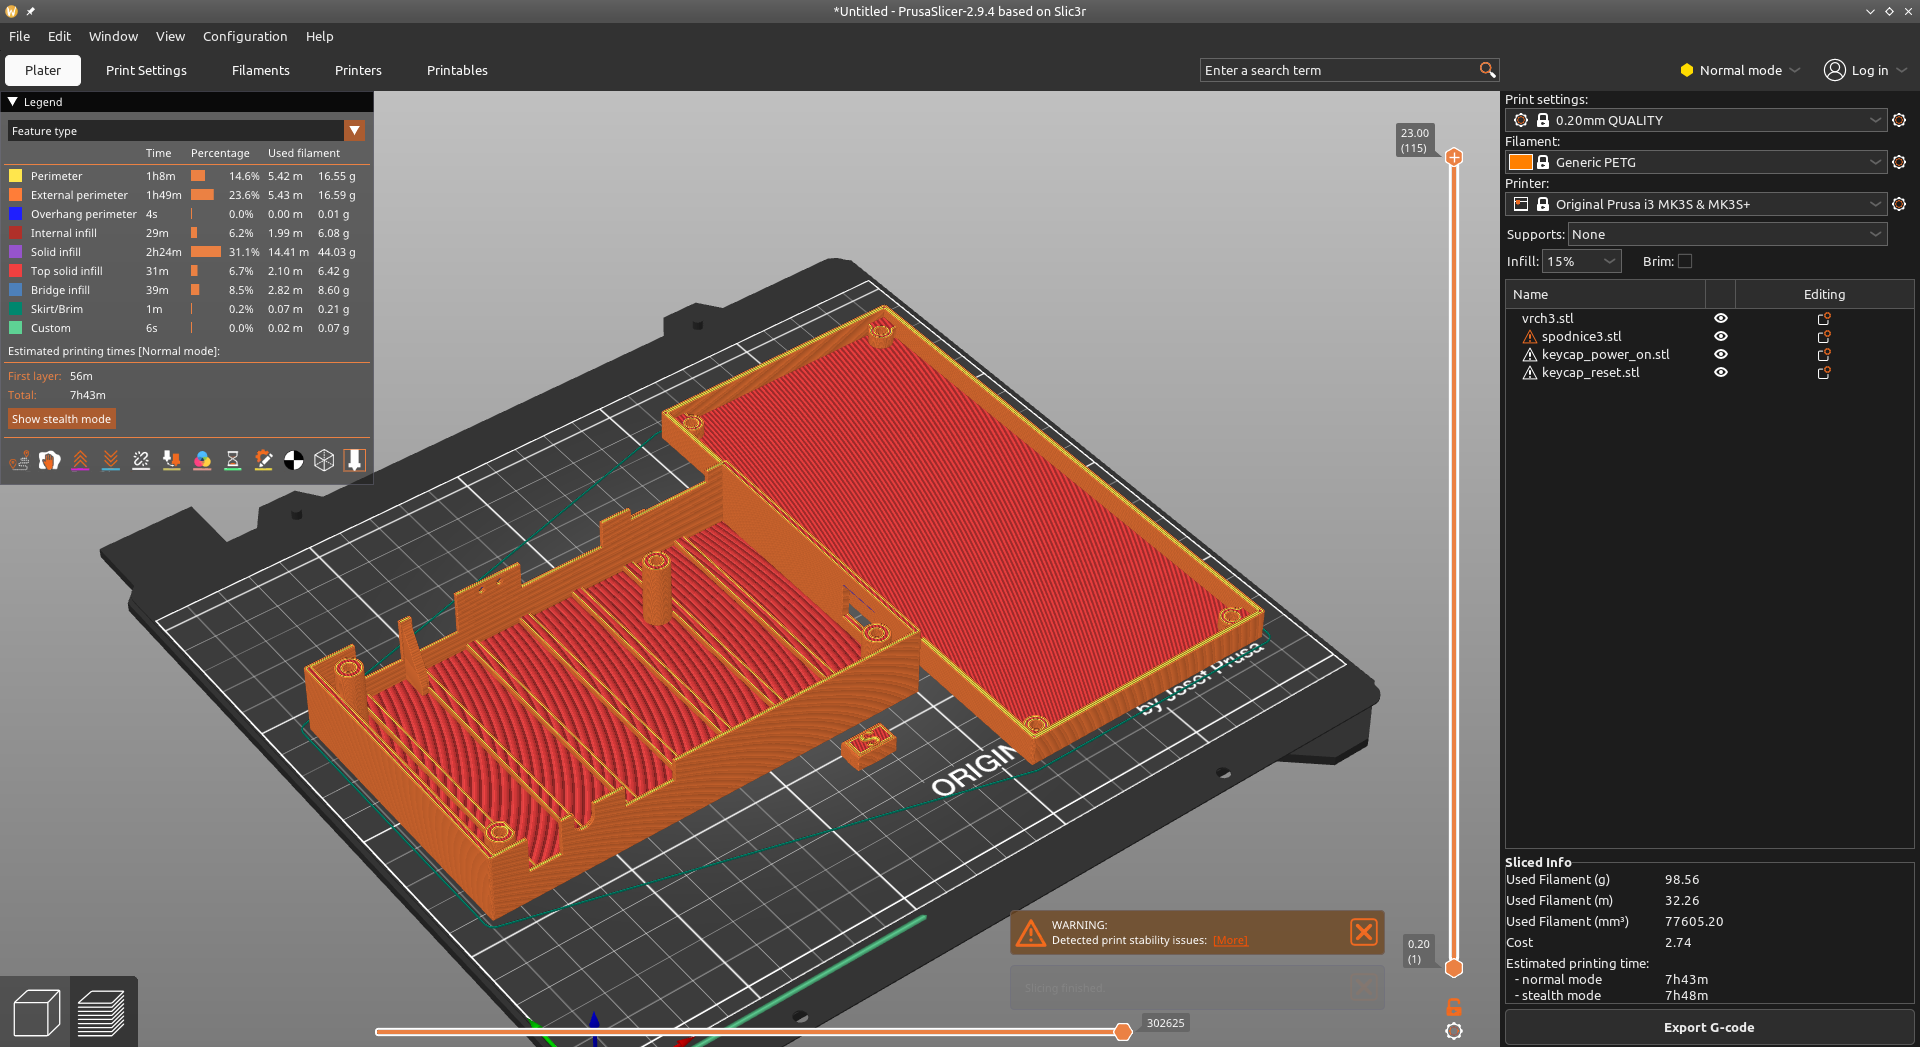
\includegraphics[width=\textwidth]{images/prusa_slicer.png}
    \caption{Příprava krytu základní desky pro 3D tisk v programu PrusaSlicer.}
\end{figure}
